%\documentclass[aps,prd,nofootinbib]{revtex4-1}
\documentclass[singlepage,notitlepage,nofootinbib,12pt]{revtex4-1}
\usepackage{amsmath}
\usepackage{graphicx}
\usepackage{subfig}
\usepackage{epsfig}
\usepackage{listings}
\usepackage[hidelinks,hyperfootnotes=false,bookmarks=false]{hyperref}
\begin{document}
\title{Problem Set 1 - G6080}
\author{Victor Genty}
%\affiliation{Department of Physics, Duke University, Durham, NC 27707, USA}
\date{\today}
%\begin{abstract}
%\end{abstract}
\maketitle
\section{Problem 1}
%\label{sec1}
The cosine recursion formula  was implemented in C++ double precision and plotted for various values of $N$ at constant $x$. The error function for an accuracy of $\epsilon_c = 10^{-15}$ in the initial guess is plotted as well as the ratio of $\Delta\cos Nx$ to the error function where,

\begin{align*}
\Delta\cos N x = \left|2\frac{\cos N x - \cos_{\text{rec}}Nx}{\cos N x + \cos_{\text{rec}}Nx}\right|,
\end{align*}
for $\cos_{\text{rec}} Nx$ and $\cos Nx$ the recursion and ``true'' IEEE double cosine respectively. We find that as N is increased from $N=10^{2}$ to $N=10^8$ the relative error in cosine from recursion follows the expected pattern and the {\it ratio} of the relative error in the recursion cosine to the error function reveals a relatively constant value varying in only a single order of magnitude. This confirms that the error in the recursion cosine follows the theoretical calculation of the error $|N\sin N x/(\sin x)\epsilon_c|$.
\begin{figure}[h]
  \centering
\subfloat[][]{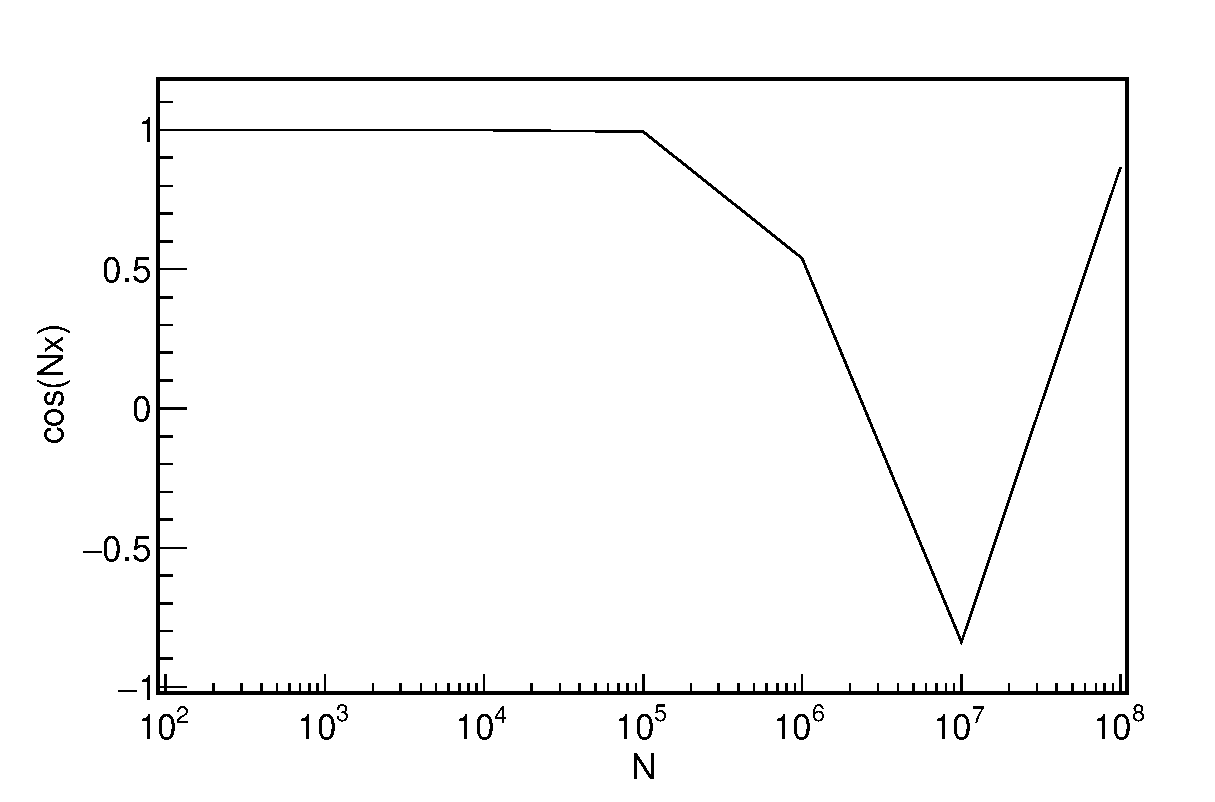
\includegraphics[width=0.5\textwidth]{figures/1a_cos.eps}}
\subfloat[][]{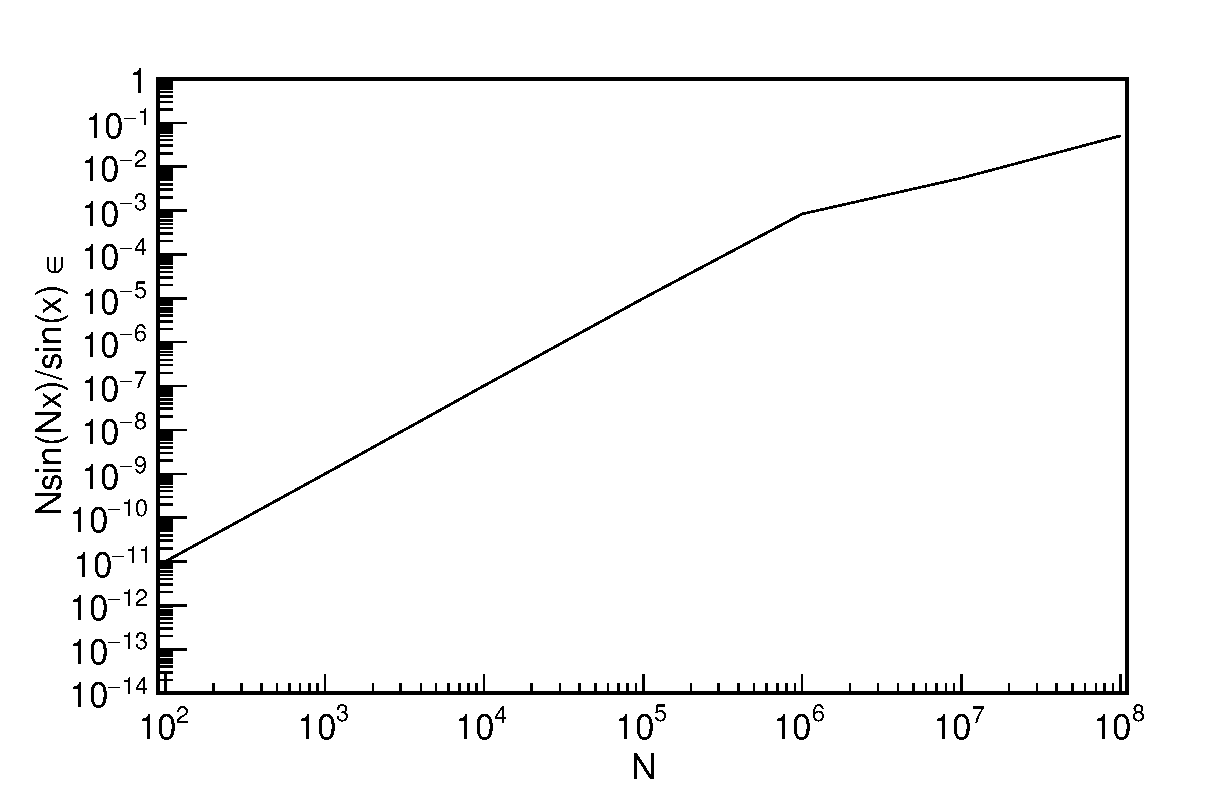
\includegraphics[width=0.5\textwidth]{figures/1a_error.eps}}\\
  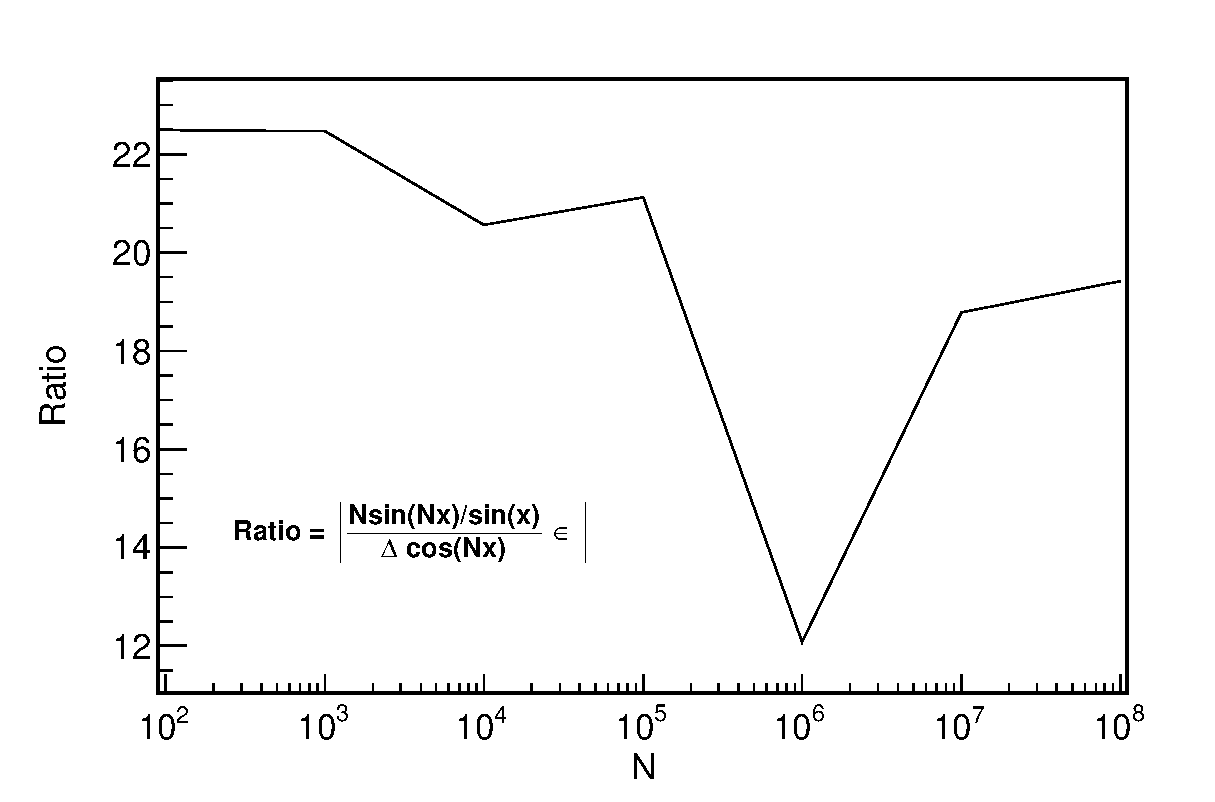
\includegraphics[width=0.5\textwidth]{figures/1a_ratio.eps}
  \hfill
  \caption{Figures for part (a) of problem 1. For each graph $x = 10^{-6}$. The left pane shows the recursion cosine at varying iterative step size $N$. THe right pane shows the theoretical error on the cosine recursion. The bottom pane shows the ratio of the relative error in the recursion cosine to the theoretical error formula.}
\end{figure}\\
\indent The formula given by equation (2) of the problem set does not include errors from the finite representation of intermediate steps in the recursion. The formula to include the errors would need to sum over the all the intermediate steps:
\begin{align*}
\frac{\Delta\cos Nx}{\cos Nx} &= \sum_{M=1}^{N-1}\frac{\partial \cos Nx}{\partial \cos Mx}\Delta\cos Nx = \sum_{M=1}^{N-1}\frac{N\sin Nx}{M\sin Mx}\cos Mx \cdot \epsilon_c\\
&= N\sin Nx\sum_{M=1}^{N-1}\frac{\cot Mx}{M} \cdot \epsilon_c.
\end{align*}
\\
\indent If we use a different accuracy for the initial value of $\cos x$ and for steps in the recursion we observe an interesting effect on the propogation of error through recursion.
\begin{figure}[h]
  \centering
\subfloat[][]{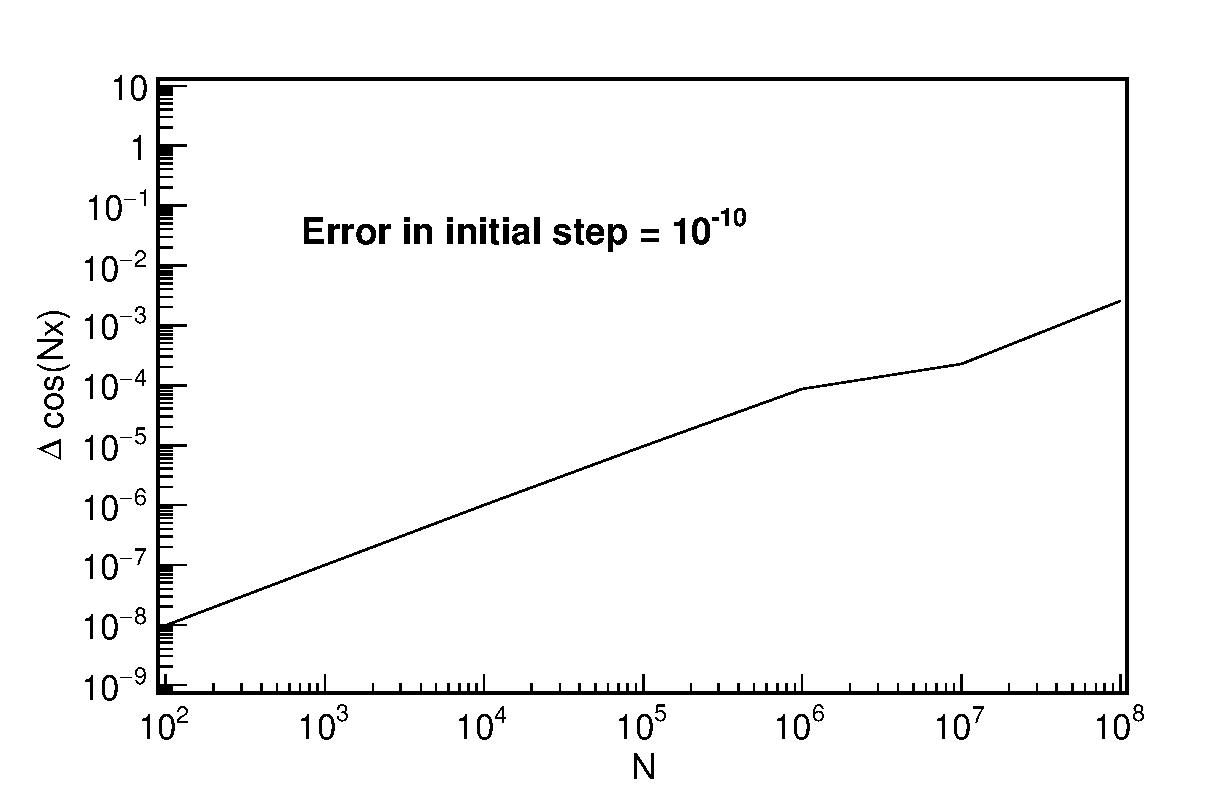
\includegraphics[width=0.5\textwidth]{figures/1c_initial.eps}}
\subfloat[][]{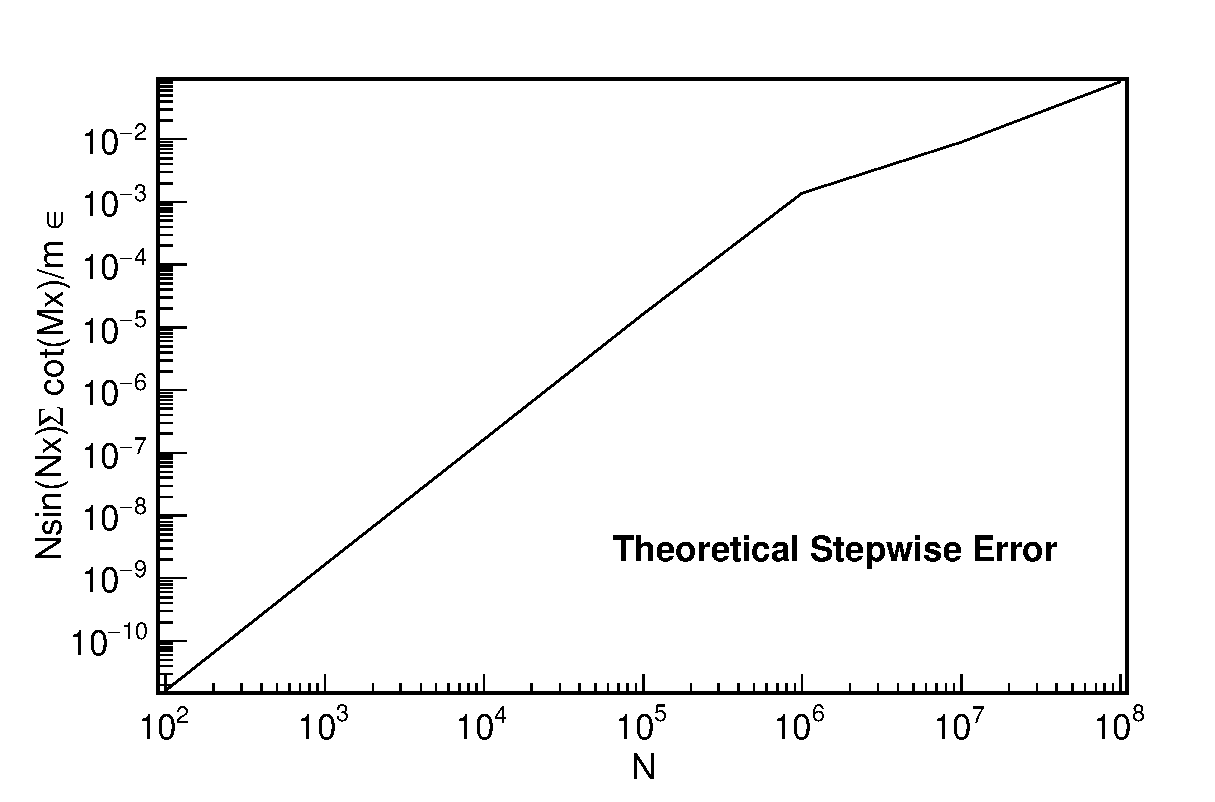
\includegraphics[width=0.5\textwidth]{figures/1c_theory_stepwise.eps}}\\
  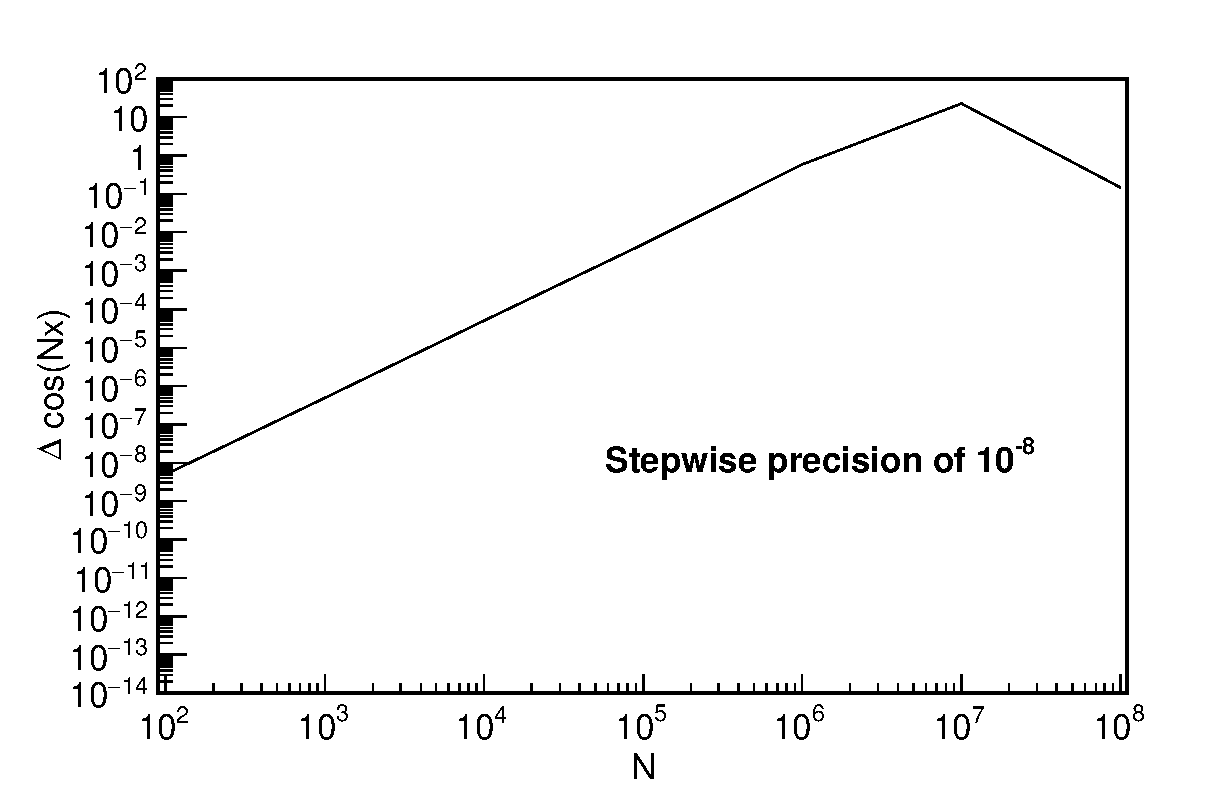
\includegraphics[width=0.5\textwidth]{figures/1c_stepwise.eps}
  \hfill
  \caption{Figures for part (c) of problem 1. For each graph $x = 10^{-6}$. The left pane shows the relative error in the recursion cosine for an error of $10^{-10}$ in the initial value. The right tpane shows the theoretical error on the stepwise error introduced from rounding/truncation between steps. The bottom plot shows the recursion cosine error with truncation.}
\end{figure}
\\
For an error in the initial calculation of cosine (the first step in the recursion) of $10^{-10}$ which is fairly large compared to IEEE double precision the expected relative error follows the expected curve. Using a high precision value of cosine for the initial value (i.e. \verb|std::cos|) and truncating each step via a function,
\begin{lstlisting}[language=C++]
  double roundd(double num) {
    return floor(num * pow(10.0,precision_) + 0.5)/pow(10.0,precision_);
  }
\end{lstlisting}
Which takes a number with N digits after the decimal place, and rounds them to \verb|precision_| decimal places. This function resembles the one found in the example script. The relative error in the recursion cosine resulting from error in each step is shown in the bottom pane where each calculation is reduced to 8 decimal places. The error does not seem to follow the expected theoretical curve as shown in the right pane above and calculated in part (b).
\section{Problem 2}
I modified the \verb|real_time_clock.c| program to calculate the 8 operations in a single execution. For each operation the program starts the clock, iterates 1000 times, stops the clock, then prints to the screen the time is took to complete the 1000 operations. At the end of the program, I calculate the overhead to start and stop the clock. A python script, \verb|two.py|, executes the modified clock program and captures the output. For each operation the python script computes the time it takes the complete one operation by dividing by the number of iterations. The script then runs the clock program 1000 times and histograms time required to complete one operation. The histograms detail the variability, or spread in binary operation time between program executions. In the histograms below, the red shaded histogram represents {\bf no} compiler optimization (\verb|gcc -O0|) and blue the {\bf highest} optimization (\verb|gcc -O3|). The number of entries in each histogram is 1000.
\begin{figure}[h]
  \centering
  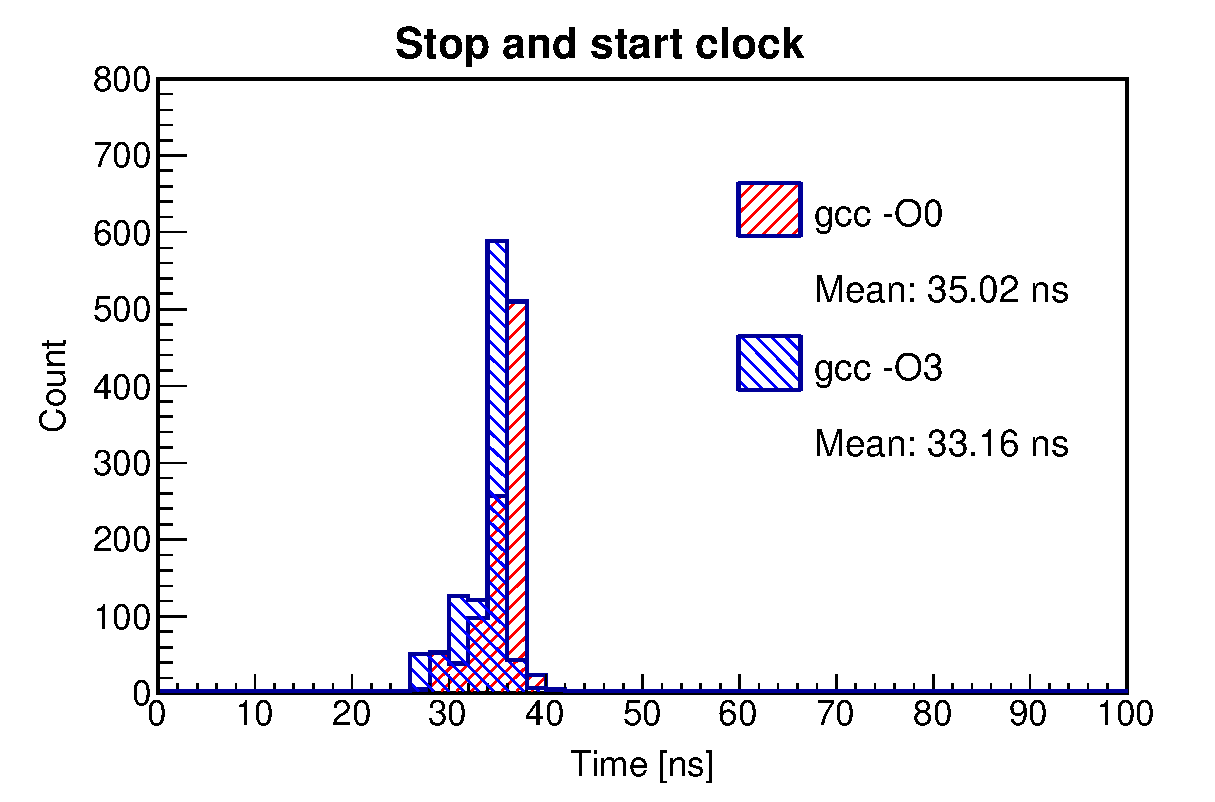
\includegraphics[width=0.5\textwidth]{figures/clock.eps}
  \subfloat[][]{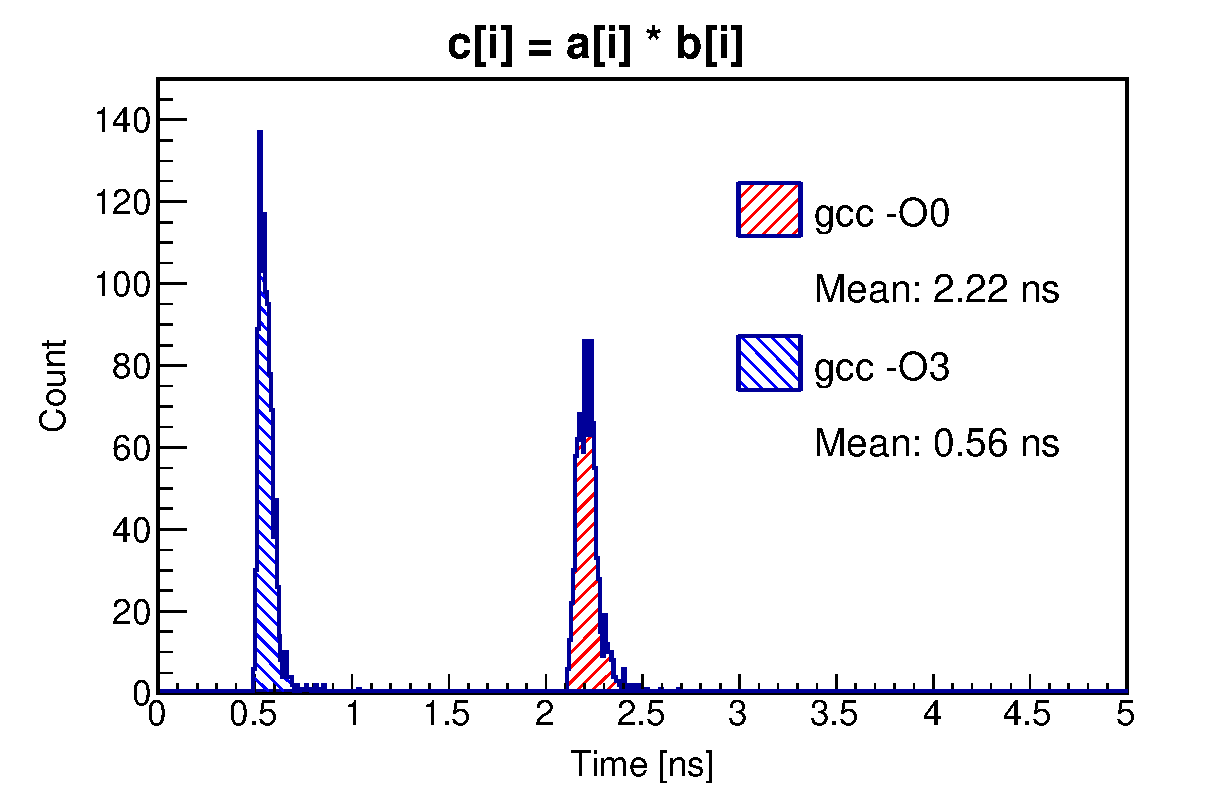
\includegraphics[width=0.5\textwidth]{figures/2_a.eps}}
  \subfloat[][]{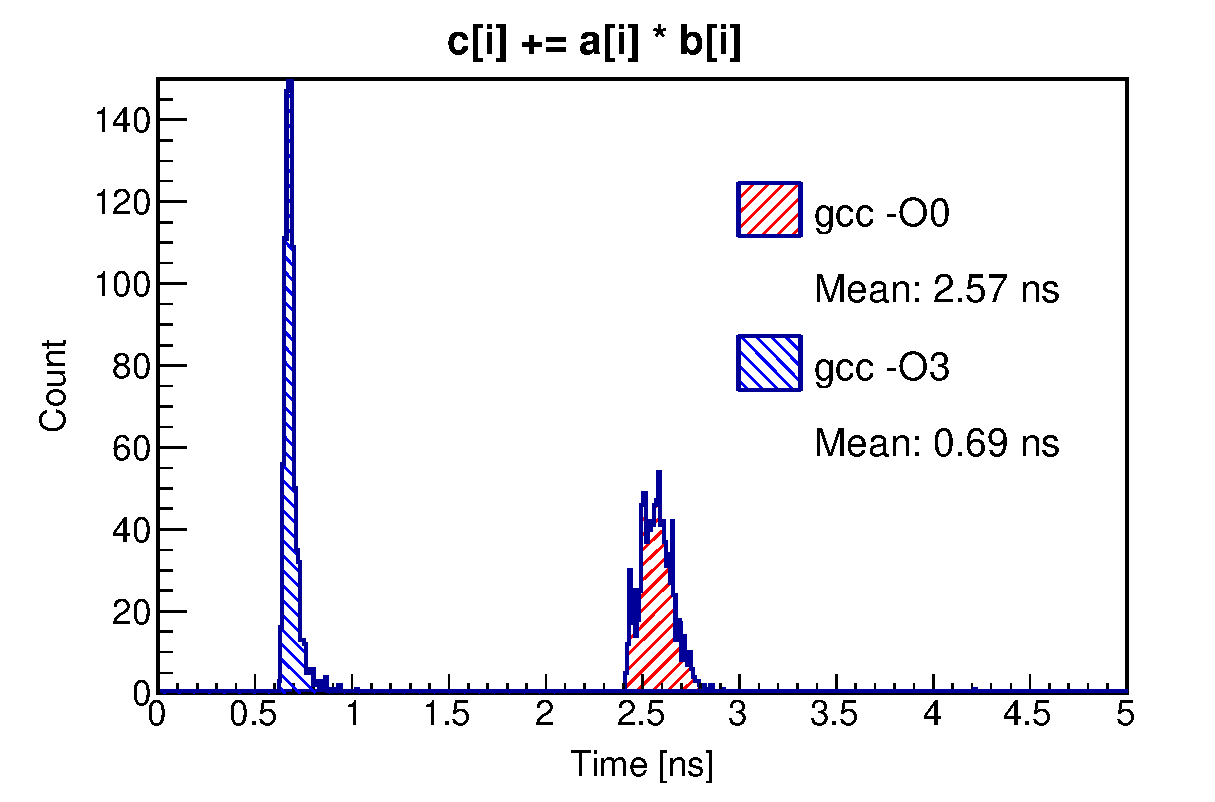
\includegraphics[width=0.5\textwidth]{figures/2_b.eps}}\\
  \subfloat[][]{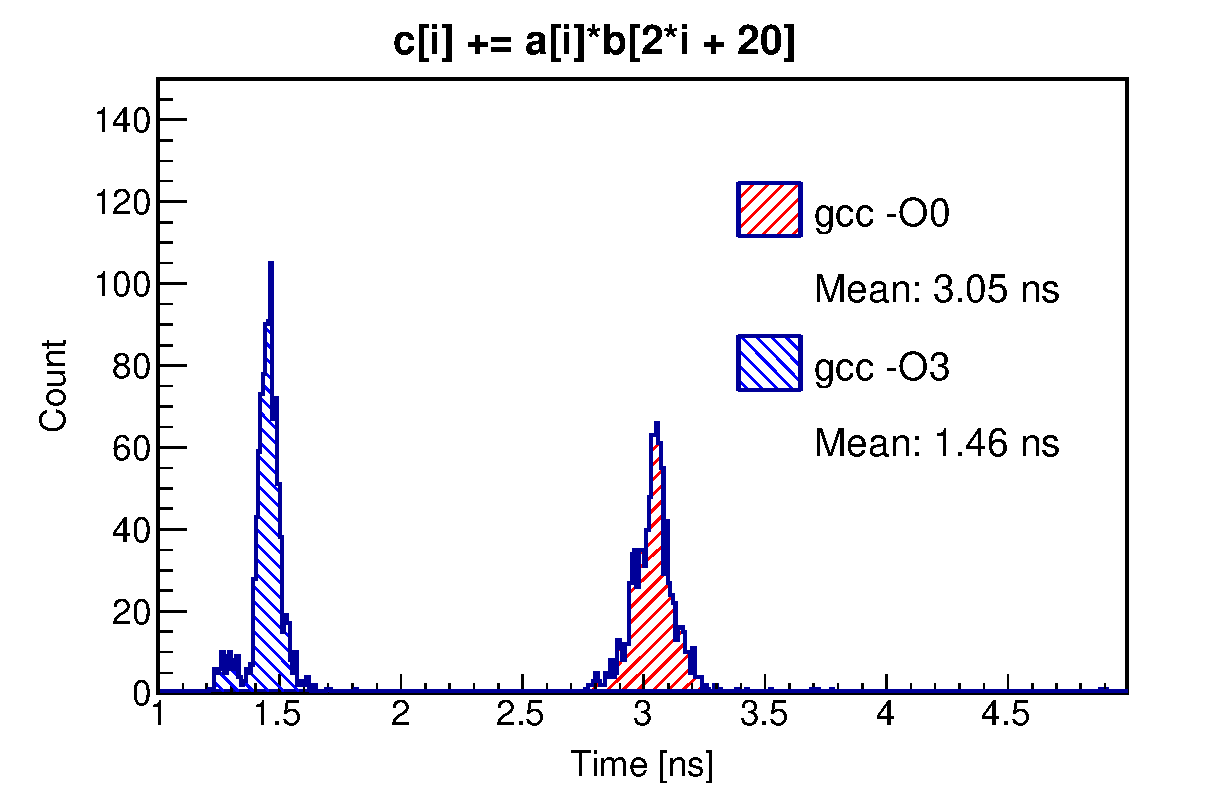
\includegraphics[width=0.5\textwidth]{figures/2_c.eps}}
  \subfloat[][]{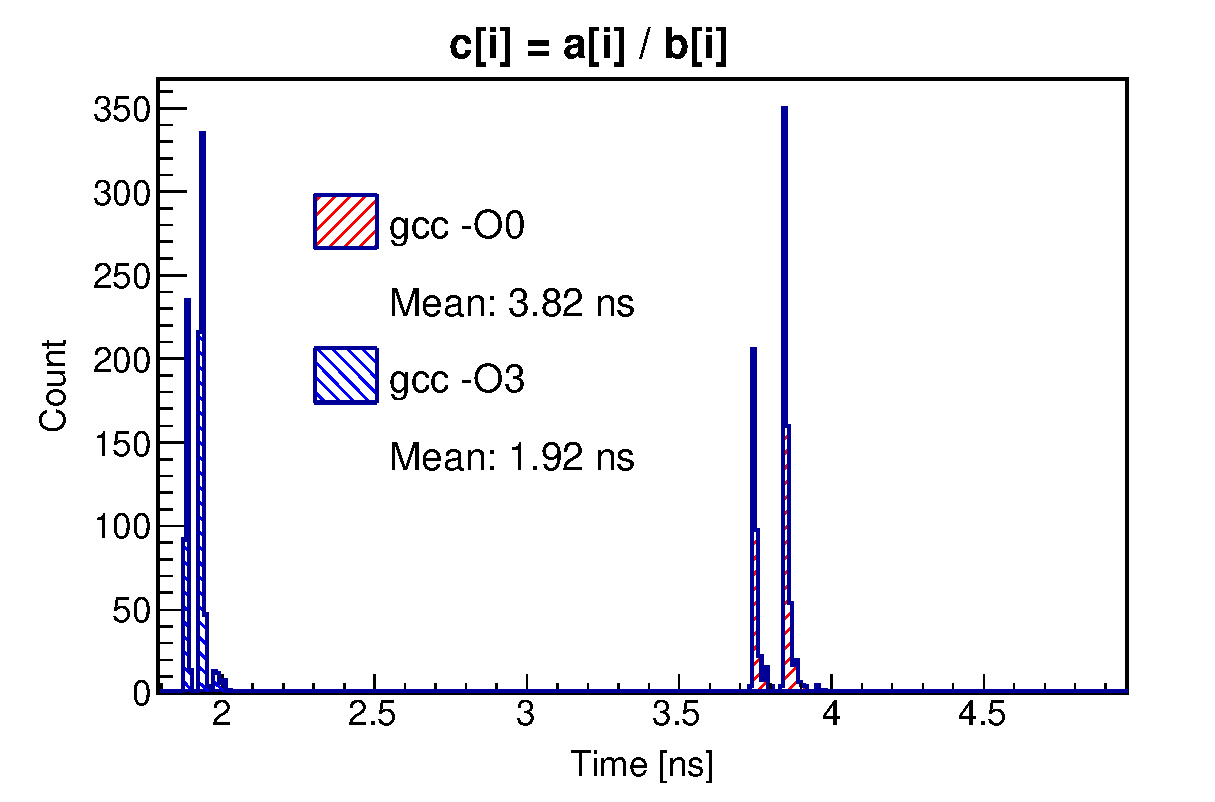
\includegraphics[width=0.5\textwidth]{figures/2_d.eps}}
\caption{Time required to execute the clock structure and parts (a) - (d) of Problem 2.}
\end{figure} 
\begin{figure}[h]
\ContinuedFloat
\centering
  \subfloat[][]{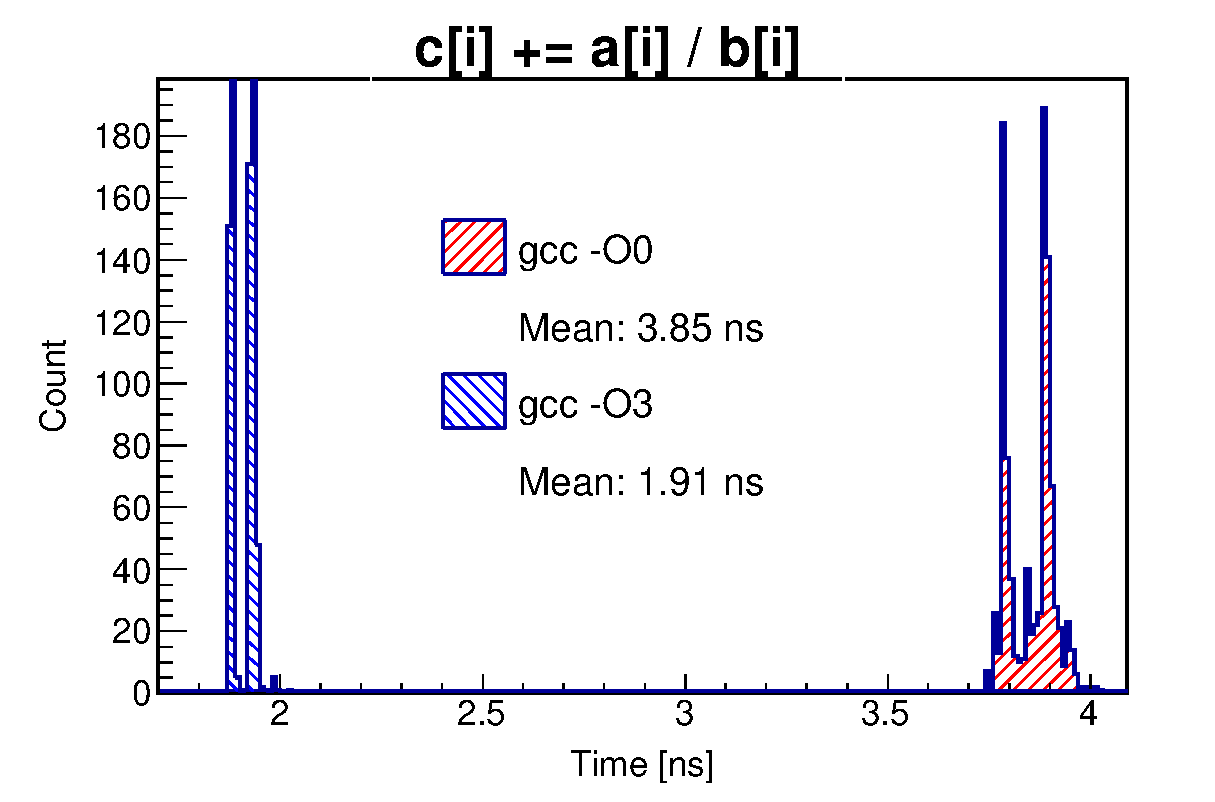
\includegraphics[width=0.5\textwidth]{figures/2_e.eps}}
  \subfloat[][]{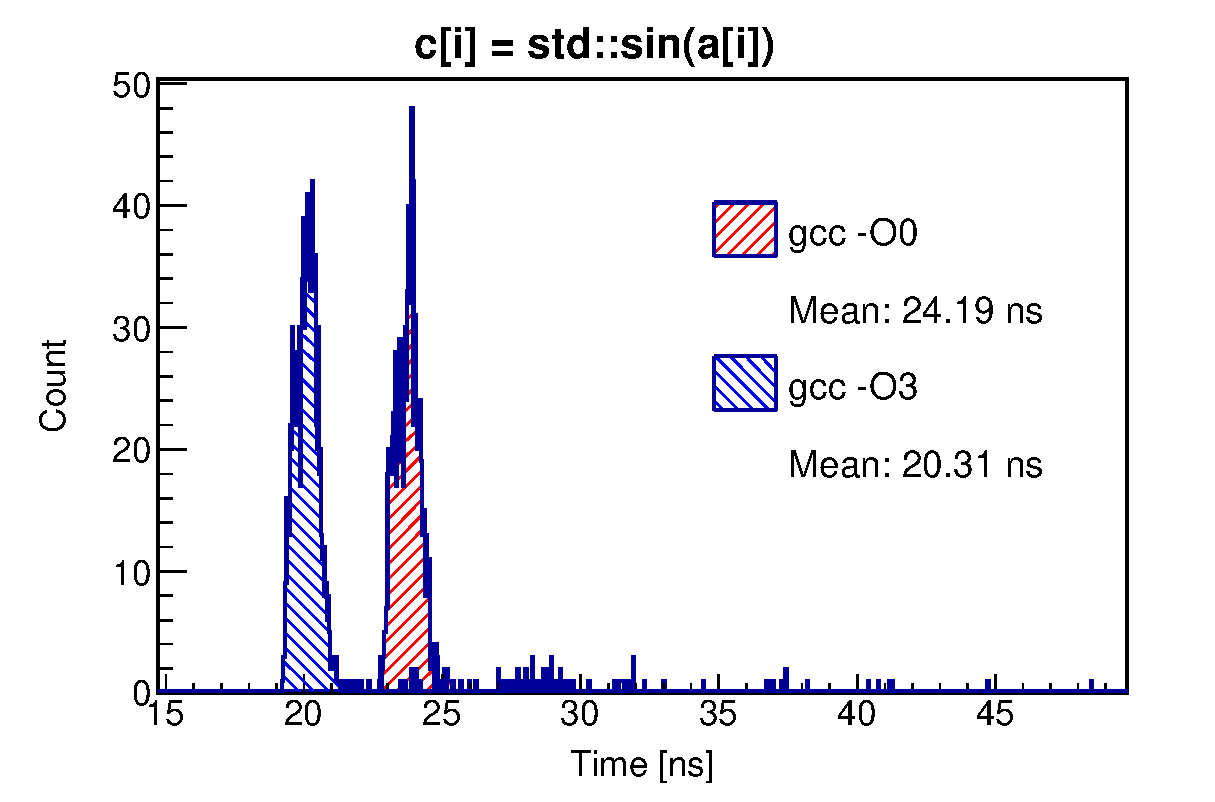
\includegraphics[width=0.5\textwidth]{figures/2_f.eps}}\\
  \subfloat[][]{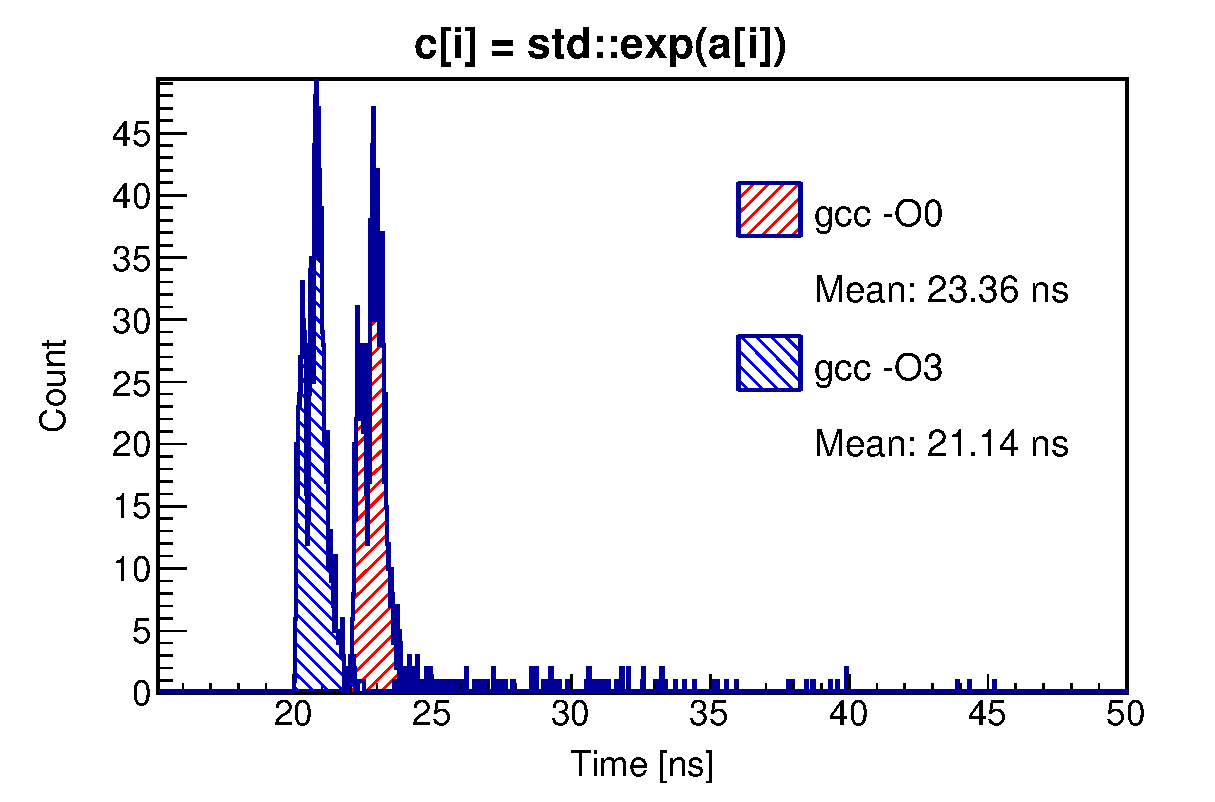
\includegraphics[width=0.5\textwidth]{figures/2_g.eps}}
  \subfloat[][]{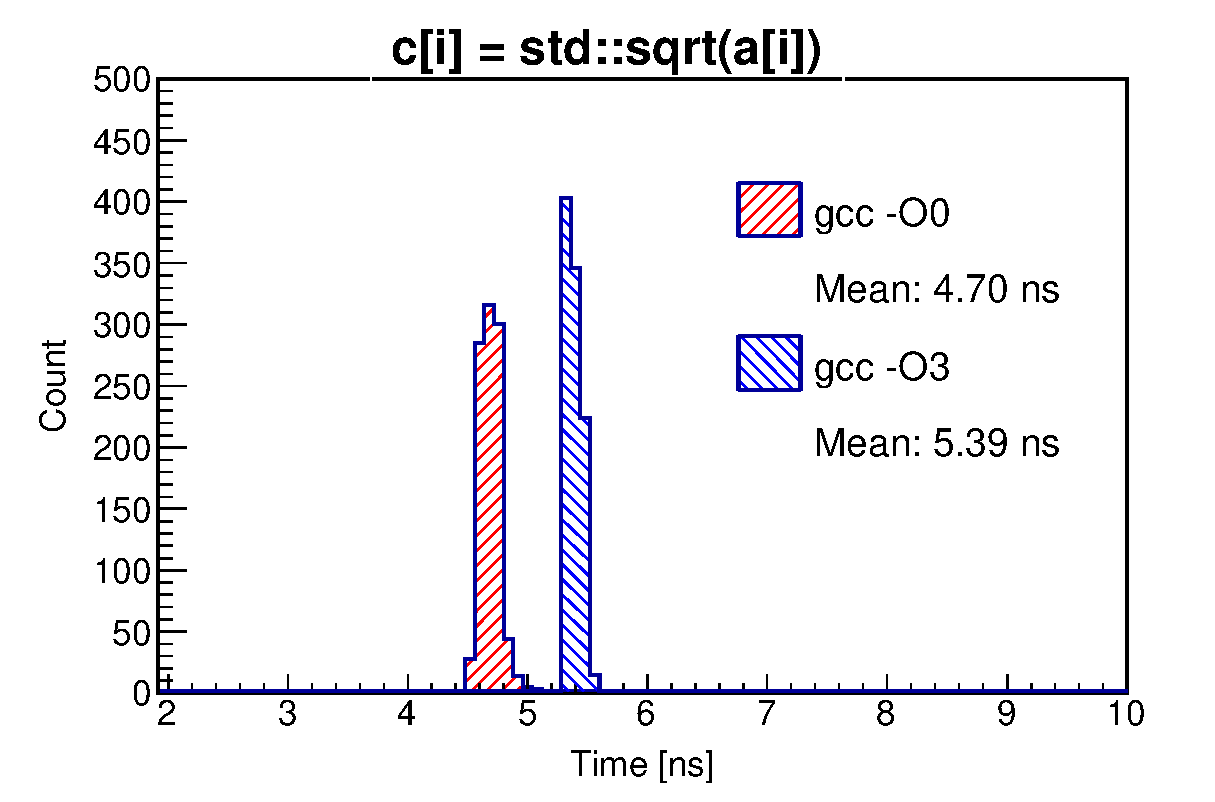
\includegraphics[width=0.5\textwidth]{figures/2_h.eps}}
\caption{Parts (e) - (h) of Problem 2.}
\end{figure}\\
\indent The overhead required to start and stop the clock was about 35 ns as shown in the first plot and did not depend too much on the compiler optimization. The fastest operation was multiplication, depending {\it heavily} on the compiler optimization which execution speed as low as half a nano-second. The slowest operations were \verb|std::sin|, and \verb|std::exp| clocking in at 20-30 ns. This likely indicates some sublayer of code is necessary to calculate analytic functions. The code was executed on Centos 7 x86\_64 with linux kernel 3.10. The hardware specfication were an Intel Core i5  3.40 GHz CPU with about 6 MB of cache. This corresponds to about a 0.3 ns/cycle. It seems like on average multiplication takes about 1-2 cycles and division on the order of 10 or so.
\clearpage
\section{Problem 3}
The modified bessel functions of the first kind $I_2(x)$ are computed for values of $x\in\{1,2,\dots,10\}$. The program \verb|Bessel| uses the C++ boost library to call the ``true'' value of the modified bessel function \verb|boost::math::cyl_bessel_i|. The program also uses variable recursion to calculate $I_2(x)$ for different value of $x$. The \verb|Bessel| program is compiled into a shared object and loaded into python via the ROOT framework. This way, python can invoke Bessel member methods at compiled speed without the interpreter overhead. The python program \verb|use.py| iterates the calculation of $I_2$ for 50 recurance steps and over 10 values of $x$. The results are plotted in the figure below. 
\begin{figure}[h]
\centering
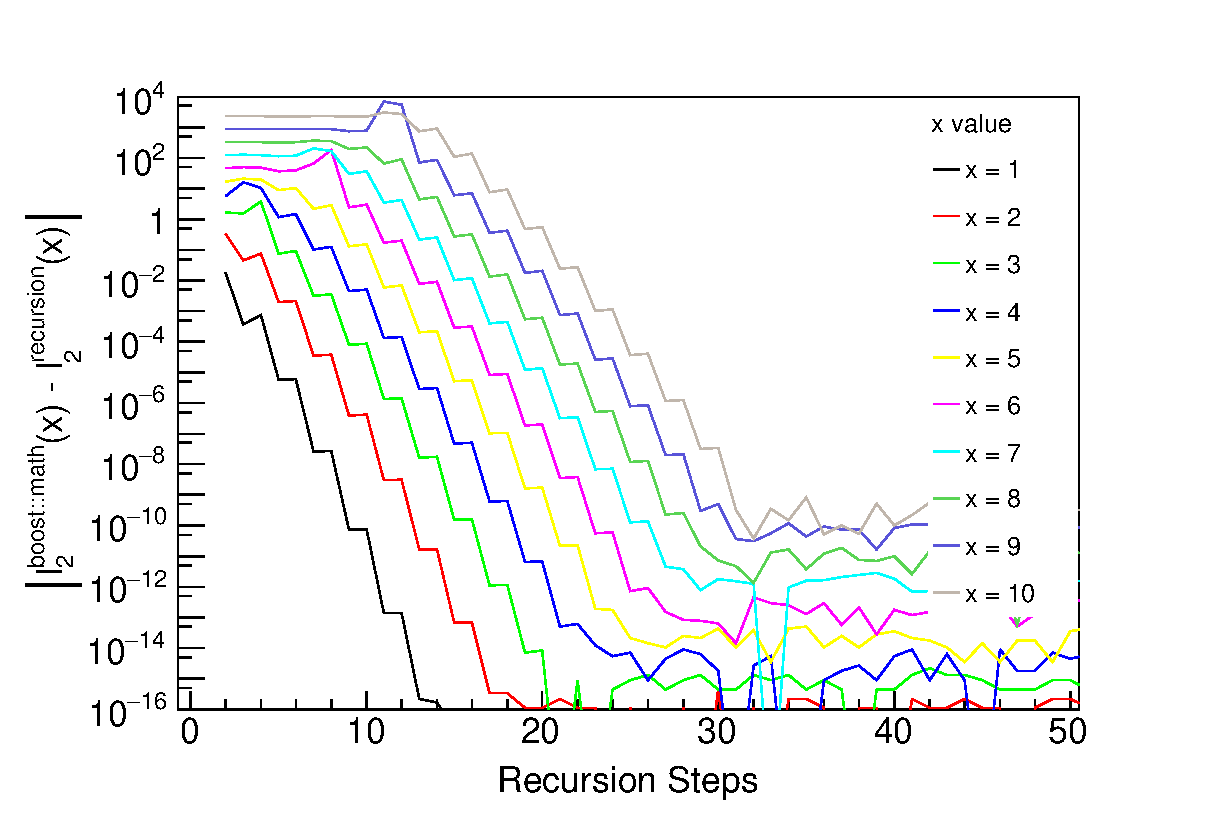
\includegraphics[width=0.6\textwidth]{figures/modified_bessel.eps}
\caption{Absolute difference between recursion modified bessel and IEEE double precision modified bessel value for varying values of $x$}
\end{figure}\\
\indent As the number of recurance steps increases, the absolute difference between the calculated value and the true (precision of $10^{-15}$) value decreases until they agree within IEEE double precision. Larger value of $x$ require more recurance steps to achieve higher precision. In addition, the agreement between the two values tends to level off about IEEE double precision. For larger value of $x$ we note that the absolute difference does not level off at precisely IEEE double precision.
\end{document}
